\chapter{Extensions}
\label{section:extensions}

\section{Solver-specific improvements}
The main principles that drive the algorithm work regardless of which solver is used. However, the implementation can be improved by using more specific features of the solver. For this thesis, IBM CPLEX is used as the MILP solver. This is one of the fastest, proprietary solvers available on the market. 

\subsection{Indicator constraints}
The Big M method to turn constraints on or off is functional, but there are some issues with it. M has to be big enough so it can always "overpower" the rest of the inequality. If M is too low, incorrect behavior may occur. However, if M is very large, CPLEX may have numerical difficulties or even find incorrect results \footnote{\url{http://www-01.ibm.com/support/docview.wss?uid=swg21400084}}. \\
Indicator constraints are a solution for this problem. The goal of the large M is to overpower the inequality so the constraint can be turned on or off based on a boolean variable. Indicator constraints allow constraints to be turned on or off, based on other constraints. They provide a direct way to model an "if/then" relation. Equation \ref{eq:indicator-obs} is a modified version of the obstacle avoidance constraints \ref{eq:obs-m-1-v} - \ref{eq:obs-m-4-v}. If $slack_{i,n}$ is not true, then the matching constraint on the right side must be true.

\begin{equation}
\label{eq:indicator-obs}
\neg slack_{i,n} \rightarrow \\
\begin{cases}
y_{n} -  v_i \quad \geq 
\quad a_{i} x_{n} + b_{i},  	
& \Delta q_{x,i} < 0 							 	
 \\
y_{n} + v_i \quad \leq 
\quad a_{i} x_{n} + b_{i},
& \Delta q_{x,i} > 0 							 	
 \\
x_{n} + r \quad \leq
\quad  q_{x,i}, 		
& \Delta q_{y,i} < 0, \quad \Delta q_{x,i} = 0 	
 \\
x_{n} - r \quad \geq 
\quad q_{y,i},  		
& \Delta q_{y,i} > 0, \quad \Delta q_{x,i} = 0 	
\end{cases}
\end{equation}

\subsection{Max time}
When the MILP problem is sufficiently difficult to solve, it may take a long time before the solver can find the optimal solution. To ensure an upper limit on computation time, CPLEX accepts a maximum solve time parameter. When the maximum time has expired, it will return the best solution found so far.\\
In the experiments, the maximum solve time was typically 120 seconds per segment. The goal is for every segment to be relatively easy to solve, so if no solution can be found in two minutes it counts as a failure.
\subsection{Max delta}
During testing it became clear that the solver often spends a relatively long time trying to improve trajectories which are already nearly optimal, or optimal but not yet proven to be optimal. CPLEX provides a maximum delta parameter. The delta is the difference between the best solution found so far and the upper bound for the optimal solution. If the delta is below this maximum delta, the solvers stop executing and returns the best result. When this value is small, this can reduce some of the execution time while barely changing the quality of the trajectory.

\section{Corner cutting}
\label{subsec:corner-cutting}
\begin{figure}
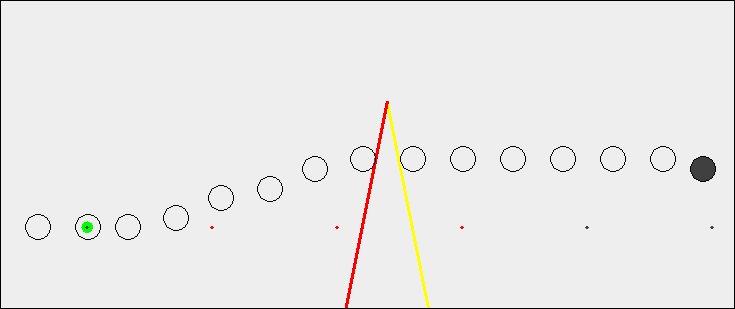
\includegraphics[width=\textwidth]{img/cornercut_bad}
\caption{An example of corner cutting}
\label{fig:cornercut-example}
\end{figure}
The MILP problem uses discrete time steps to model the changes in the UAV's state over time. An issue with this approach is that constraints are only enforced at those specific time steps. This allows the UAV to cut corners or even move through obstacles entirely if the vehicle is moving fast enough. Figure \ref{fig:cornercut-example} shows an example of this. Each time step on its own is a valid position, but a collision is ignored between the time steps.\\
Using the indicator constraint notation, Equation \ref{eq:obs-repeat-1} and \ref{eq:obs-comb-repeat-1} prevent collisions with obstacle $o$ at time step $n$. Each edge of each obstacle has an associated $slack$ variable, which determines whether or not the UAV is on the safe side for that edge.
\begin{equation}
\label{eq:obs-repeat-1}
\neg ~ slack_{i,n} \rightarrow \\
\begin{cases}
y_{n} -  v_i \quad \geq 
\quad a_{i} x_{n} + b_{i},  	
& \Delta q_{x,i} < 0 							 	
 \\
y_{n} + v_i \quad \leq 
\quad a_{i} x_{n} + b_{i},
& \Delta q_{x,i} > 0 							 	
 \\
x_{n} + r \quad \leq
\quad  q_{x,i}, 		
& \Delta q_{y,i} < 0, \quad \Delta q_{x,i} = 0 	
 \\
x_{n} - r \quad \geq 
\quad q_{y,i},  		
& \Delta q_{y,i} > 0, \quad \Delta q_{x,i} = 0 	
\end{cases}
\end{equation}
\begin{equation}
\label{eq:obs-comb-repeat-1}
\neg \mathlarger{\mathlarger{\bigwedge_{i}}} slack_{i,n} \quad 0 \leq n \leq N
\end{equation}
Richards and Turnbull\cite{Richards2015} proposed a method which prevents corner cutting. In their method, the UAV is consider on the safe side of an edge only if that is true for two consecutive time steps.  This is visualized in Figure \ref{fig:cc-fixed}. They apply the same constraints again, but this time on the position of the UAV in the last time step:
\begin{equation}
\label{eq:corner-skip-fixed}
\neg ~ slack_{i,n} \rightarrow \\
\begin{cases}
y_{n-1} -  v_i \quad \geq 
\quad a_{i} x_{n-1} + b_{i},  	
& \Delta q_{x,i} < 0 							 	
 \\
y_{n-1} + v_i \quad \leq 
\quad a_{i} x_{n-1} + b_{i},
& \Delta q_{x,i} > 0 							 	
 \\
x_{n-1} + r \quad \leq
\quad  q_{x,i}, 		
& \Delta q_{y,i} < 0, \quad \Delta q_{x,i} = 0 	
 \\
x_{n-1} - r \quad \geq 
\quad q_{y,i},  		
& \Delta q_{y,i} > 0, \quad \Delta q_{x,i} = 0 	
\end{cases}
\end{equation}
\begin{figure}
	\centering
	\begin{subfigure}[t]{0.3\columnwidth}
        		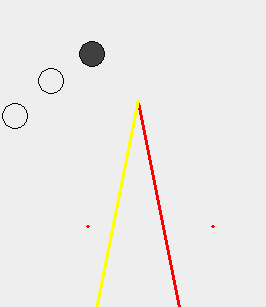
\includegraphics[width=\textwidth]{cornercut-fixed-1}
        		\caption{}
        		\label{fig:cc-fixed-1}
	\end{subfigure}
	\hfil
	\begin{subfigure}[t]{0.3\columnwidth}
        		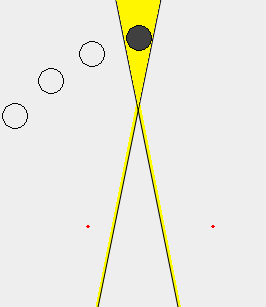
\includegraphics[width=\textwidth]{cornercut-fixed-2b}
        		\caption{}
        		 \label{fig:cc-fixed-2}
	\end{subfigure}	
		\hfil
	\begin{subfigure}[t]{0.3\columnwidth}
        		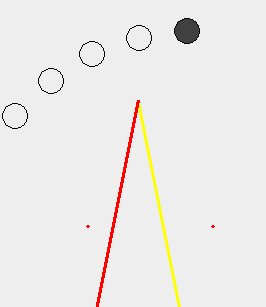
\includegraphics[width=\textwidth]{cornercut-fixed-3}
        		\caption{}
        		\label{fig:cc-fixed-3}
	\end{subfigure}
    \caption{These images are three consecutive time steps which demonstrate how the corner cutting prevention works. In \ref{fig:cc-fixed-1}, the UAV is in the safe region of the left edge (which is indicated by the yellow color). In \ref{fig:cc-fixed-3}, the UAV is in the safe region for the right edge, but not the left edge. To ensure that the UAV does not cut the corner, the UAV must enter the safe region of the right edge before it exits the safe region of the left edge. The intersection between those two safe regions is the inverted yellow triangle in \ref{fig:cc-fixed-2}. If the UAV spends at least one time step in that yellow, it cannot cut the corner.}
    \label{fig:cc-fixed}     
\end{figure}

\section{Stability Improvements}

\subsection{Maximum goal velocity}
\begin{figure}[]
	\centering
	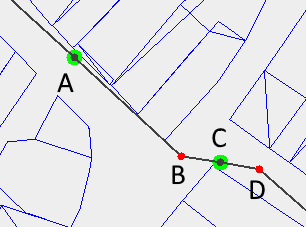
\includegraphics[width=0.5\textwidth]{goalvel}
	\caption{A visual demonstration of when a maximum goal velocity is used. Points B and D are individual turn events. The segment for event B starts at A, with |AB| being the desired expansion distance for the segment. However, because D is so close to B, the end of the segment C cannot be placed at the desired expansion distance from B. Instead, C is placed in the middle between B and D, such that |BC|=|CD|. The first segment solves the trajectory from A to C past turn event B, the second segment starts as C, past D and onwards. The goal is to ensure that the UAV can still safely stop at D when it starts the second segment at C. This is done by limiting the maximum velocity of the UAV when it reaches the goal C in the first segment.}
	\label{fig:max-goal-vel}
\end{figure}

When two corners are close to each other, it may not be possible to expand each corner outwards by the full expansion distance. In that case, the middle between those corners is chosen as the transition between the the segments for each corner. \\
This ensures that both corners get a fair share of the space between them. However, it breaks the assumption behind the corner expansion. If the velocity after the first corner is high, due to the reduced approach distance, the UAV may not be able to stop in time for the corner. In this situation, no solution will be found in the second segment. Figure \ref{fig:max-goal-vel} shows a situation when this may be necessary.\\
As a solution for this, the UAVs velocity at the goal of the first segment can be limited so it can stop in time for the corner in the next segment. The maximum distance at the goal of the segment is $v'_{max}$, given the actual expansion distance $dist$ in Equation \ref{eq:goalvel}. 

\begin{equation}
\label{eq:goalvel}
v'_{max} = \sqrt{2 * dist * a_{max}}
\end{equation}

\subsection{GA start area}
\begin{figure}
	\centering
	\begin{subfigure}[t]{0.45\columnwidth}
        		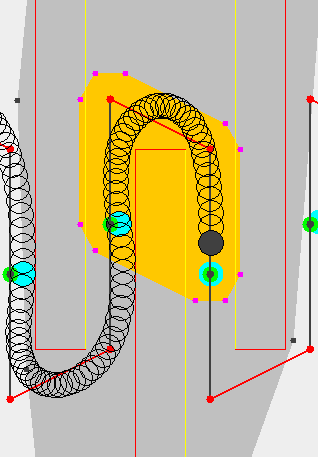
\includegraphics[width=\textwidth]{limited-ga-seed}
        		\caption{}
        		\label{fig:ga-seed-pre}
	\end{subfigure}
	\hfil
	\begin{subfigure}[t]{0.45\columnwidth}
        		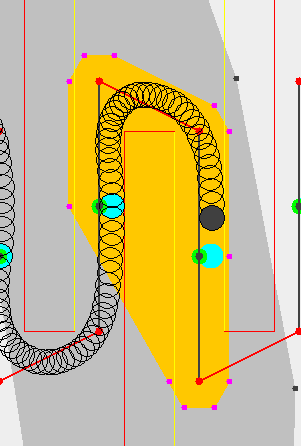
\includegraphics[width=\textwidth]{extended-ga-seed}
        		\caption{}
        		 \label{fig:ga-seed-post}
	\end{subfigure}	
    \caption{}
    \label{fig:ga-seed}     
\end{figure}
not just path: stop point based on start state
stop point based on  maximum goal velocity and goal: ensures vehicle can stop in next segment

\subsection{Goal conditions}
\begin{figure}[]
	\centering
	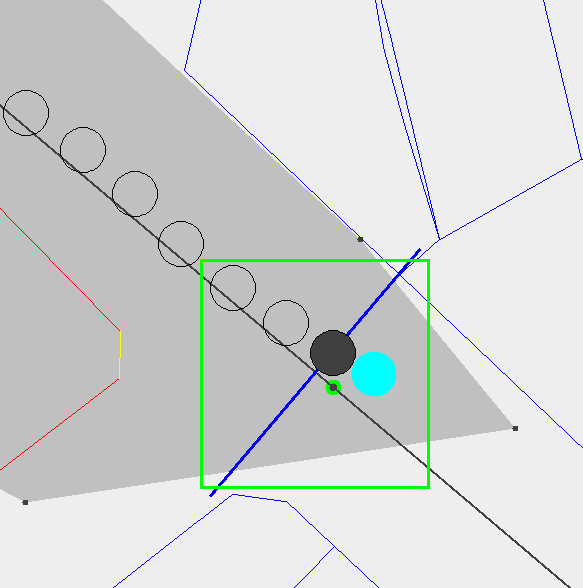
\includegraphics[width=0.5\textwidth]{segment-extend-goal-zoom}
	\caption{REPLACE! square is offset}
	\label{fig:extended-goal-zoom}
\end{figure}

larger epsilon on goal condition
prevent uav from finishing early -> use line

\section{Overlapping segment transitions}
overlap...
